\documentclass{article}
\usepackage[a4paper,margin=1in]{geometry}

\title{Fast and accurate protein false discovery rates on large-scale
proteomics data sets with Percolator 3.0}

\author{Matthew The\\
Science for Life Laboratory\\
School of Biotechnology\\
Royal Institute of Technology - KTH\\
Box 1031, 17121 Solna\\ Sweden
\and 
Michael J. MacCoss\\
Department of Genome Sciences\\
School of Medicine\\
University of Washington\\
Seattle, Washington 98195\\
United States of America
\and 
William S. Noble\\
Department of Genome Sciences\\
School of Medicine\\
University of Washington\\
Seattle, Washington 98195\\
United States of America
\and
Lukas K\"{a}ll\\
Science for Life Laboratory\\
School of Biotechnology\\
Royal Institute of Technology - KTH\\ 
Box 1031, 17121 Solna\\ Sweden}

\usepackage{setspace}
\usepackage{amsmath}
\usepackage{url}
\usepackage{graphicx}
\usepackage[outdir=./img/]{epstopdf}
\usepackage{epsfig}

\begin{document}

\maketitle

\doublespacing

Keywords: mass spectrometry - LC-MS/MS, statistical analysis, 
data processing and analysis, protein inference, large-scale studies


\newpage

\begin{abstract} 

Percolator is a widely used software tool that increases yield in
shotgun proteomics experiments and assigns reliable statistical
confidence measures, such as $q$~values and posterior error
probabilities, to peptides and peptide-spectrum matches (PSMs) from
such experiments. Percolator's processing speed has been sufficient
for typical data sets consisting of hundreds of thousands of
PSMs. With our new scalable approach, we can now also analyze millions
of PSMs in a matter of minutes on a commodity computer.  Furthermore,
with the increasing awareness for the need for reliable statistics on
the protein level, we compared several easy-to-understand protein
inference methods and implemented the best-performing
method---grouping proteins by their corresponding sets of theoretical
peptides and then considering only the best-scoring peptide for each
protein---in the Percolator package. We used Percolator 3.0 to analyze
the data from a recent study of the draft human proteome containing 25
million spectra (PM:24870542).

The source code and Ubuntu, Windows, MacOS and Fedora binary packages
are available from \url{http://percolator.ms/}
under an Apache 2.0 license.
\end{abstract}

\newpage

\section*{Introduction}

Percolator~\cite{kall2007} has played a prominent part in the analysis
pipelines of shotgun proteomics experiments for the last decade, as a
post-processor of the results from database search engines such as
SEQUEST~\cite{eng1994}, MASCOT~\cite{cottrell1999},
X!~Tandem~\cite{craig2004tandem} and MS-GF+~\cite{kim2008}. Not only
does Percolator provide a significant boost in the number of
statistically significant peptide-spectrum matches (PSMs) or peptides,
it also provides a consistent statistical framework in which to
interpret the search results. Because Percolator's running time is
usually much lower than that of the search engine, applying it as a
post-processing step should be the default choice when processing
shotgun proteomics data. As part of the continuous development and
support of the Percolator package, we present two major additions
aimed at supporting analysis of large scale proteomics studies.

First, as advances in technology continue to reduce the cost and
effort needed to carry out shotgun proteomics experiments, the amount
of data per study will keep rising steadily. While previous versions
of Percolator are able to process the data from the vast majority of
current studies in a reasonable time frame, the algorithm has some
limitations for laboratories without access to a high-performance
computing facility. When processing millions of PSMs, the majority of
Percolator's processing time is spent on training support vector
machine (SVM) classifiers.  In some settings, however, the performance
of the SVM as a function of the size of its training set plateaus at
a relatively low number of input PSMs~\cite{gonnelli2015decoy}. Here,
we use Percolator's semi-supervised learning algorithm to train SVMs
on a randomly selected subset of the PSMs and use the resulting score
vectors to evaluate the rest of the PSMs.  This random downsampling
approach yields much shorter analysis times without any loss in
statistical power.

Second, we have investigated efficient ways to obtain protein-level 
accuracy estimates. One of the major obstacles was the question of how 
to deal with shared peptides and protein grouping. An implementation 
of Fido~\cite{serang2010efficient}, which has been part of the 
Percolator package since 2012, addresses these two issues but is too 
computationally expensive to apply to large-scale data sets. We 
therefore compared four straightforward and scalable protein inference 
methods: using the best-scoring peptide, the two-peptide 
rule~\cite{carr2004need, gupta2009false}, the product of 
peptide-level posterior error probabilities (PEPs), and Fisher's 
method for combining independent $p$~values.

Although each of these methods is efficient to compute, they each 
offer specific pros and cons. Savitski {\em et 
al.}~\cite{savitski2015scalable} showed that, on large-scale data 
sets, taking the best-scoring peptide as the representative of a 
protein was superior to incorporating information from lower-scoring 
peptides. However, this approach is unsatisfying because the method 
discards all information but the best-scoring PSM for each protein. A 
simple way to combine evidence at the peptide level is the widely used 
two-peptide rule.  This approach requires evidence for a second 
peptide to support a protein inference, thereby preventing so-called 
``one-hit wonders'', {\em i.e.}, cases where a single, potentially 
spurious PSM yields a spurious protein detection. An alternative that 
takes into account even more evidence is to compute the product of 
peptide-level PEPs. This procedure takes into account all peptides 
within a protein and provides some protection against one-hit 
wonders~\cite{cox2008maxquant}. The method also has the benefit that 
correctly inferred proteins are not strongly affected by incorrectly 
inferred peptides, because these typically contribute a multiplicative 
term that is close to $1.0$. However, a concomitant drawback to using 
the product of PEPs is that it is not clear how to scale the resulting 
product to take into account protein length. Also, it is not obvious 
{\em a priori} that the independence assumption implicit in taking the 
product applies in this case.  The latter concern also applies to 
Fisher's method, which is a classical technique for combining 
independent $p$~values~\cite{fisher1925statistical}. Like the product 
of PEPs, Fisher's method takes into account all peptides of a protein, 
penalizing one-hit wonders on the basis of their many accompanying 
incorrect peptide inferences~\cite{spirin2011assigning, alves2015mass, 
granholm2013determining}.  This last characteristic can however also 
be a disadvantage, as many incorrect peptide inferences can overrule a 
minority of correct peptide inferences.  Unlike the product of PEPs, 
Fisher's method explicitly accounts for the number of $p$~values being 
combined and hence normalizes for protein length.

\section*{Methods}

We downloaded three sets of spectra, two from large-scale studies on
human samples with several millions of spectra and one smaller-scale
study on yeast samples.

The first large-scale set comprises $2212$ runs on $17$ adult tissues,
$7$ fetal tissues, and $6$ hematopoietic cell types with a total of
${\sim}25$ million spectra~\cite{kim2014draft}. The samples were
analyzed on an LTQ Orbitrap Velos and Elite (Thermo Scientific)
equipped with an Easy-nLC II nanoflow LC systems (Waters). We will
refer to this set as the Kim data set.

The second large-scale set was taken from a study aimed at studying
variation of protein abundance in human~\cite{wu2013}. It consists
of $561$ runs on $51$ samples from lysates of lymphoblastoid cell
lines, resulting in ${\sim}9$ million spectra. The peptides were
labelled with TMT 6-plex to enable quantification. The analysis took
place on an LTQ Orbitrap Velos (Thermo Scientific) equipped with an
online 2D nanoACQUITY UPLC system (Waters). We will refer to this set
as the Wu data set.

For verification of the accuracy of protein-level false discovery rate 
(FDR) estimates we additionally downloaded $92\,974$ spectra from 
three injections of yeast cells grown to mid-log phase, collected on 
an LTQ Orbitrap Velos (Thermo Scientific), as described in Moruz {\em 
et al.}~\cite{moruz2013}.  We will refer to this set as the 
``hm\_yeast'' set.

Converting the RAW files to two separate files in the MS1 and MS2 
formats~\cite{mcdonald2004ms1} respectively was done with 
ProteoWizard~\cite{kessner2008} with vendor peak picking for the MS2 
spectra and all other options left at their default values.  Next, we 
assigned high-resolution precursor masses and charges using 
information from the precursor scans with Hardkl\"{o}r 
\cite{hoopmann2007} followed by Bullseye \cite{hsieh2009}, both with 
the default parameters, through the Crux 2.0 package 
interface~\cite{mcilwain2014}.

For the Kim data set, the data was searched against the human
Swiss-Prot and Swiss-Prot+TrEMBL databases
(\url{http://www.uniprot.org/}, accessed: 2015 Nov 12)
concatenated with a database of common contaminants (source:
\url{http://maxquant.org/contaminants.zip}, accessed: 2015 Apr 17)
using the Tide search engine, again through the Crux interface. We
used semi-tryptic searches and Tide's default fragment tolerance. The
other search parameters were kept the same as in~\cite{kim2014draft}
(10~ppm precursor window, up to two missed cleavages, up to two
oxidations of methionine per peptide, variable acetylation of
N-termini), except that we did not include variable modifications for
the cyclization of N-terminal glutamine. 

For the Wu data set, we searched the spectra against the IPI Human
database version 3.74 (\url{http://www.ebi.ac.uk/IPI}, accessed: 2014
May 22) using the Tide search engine through the Crux interface. We
used Tide's default fragment tolerance, and the other search
parameters were kept the same as in~\cite{wu2013} (10~ppm precursor
window, up to two missed cleavages, up to two oxidations of methionine
per peptide, variable TMT labeling (229.16293 Da) of lysine and
N-terminal amino acids).

The target protein sequences were reversed to construct a decoy 
protein database, and separate searches were done on the target and 
decoy protein database for input to Percolator 3.0. We calculated 
protein-level FDR estimates using the picked target-decoy strategy for 
all methods~\cite{savitski2015scalable}. Unless stated otherwise, 
Percolator was run with the default parameters, which includes 
target-decoy competition on the PSMs.

\subsection*{Subset training}

By default, Percolator's semi-supervised learning algorithm randomly 
splits the list of PSMs into three subsets, {\em i.e.} the 
cross-validation bins, and trains three separate SVM classifiers, each 
trained on two of the three subsets and tested on the remaining 
subset. Each SVM classifier produces a scoring vector, which can then 
be used to calculate a new score for each PSM based on its feature 
set. The final scores are thus calculated using the classifier for 
which the PSM was in the test set.

To implement subset training, we used a downsampling strategy in which 
we randomly sample a subset of the PSM. Subsequently, we applied 
Percolator's normal training algorithm to this subset, resulting in 
three SVM classifiers in the same fashion as mentioned above. For each 
PSM, including those not selected for training, we then calculated its 
score as the average of the scores from each of the three SVMs. This 
strategy involves some overlap between training and test sets, because 
PSMs selected as part of the training subset will be evaluated by two 
SVM classifiers which were trained on this particular PSM, and will 
only avoid problems of overfitting when the strategy is carried out on 
large data sets. This strategy was adopted for simplicity of 
implementation. In a future version of the code, we will implement a 
scheme in which we downsample each cross-validation bin individually.

Preliminary results showed that including target and decoy PSMs 
belonging to the same spectrum together during the selection of the 
random subset gave more stable performance than sampling without 
taking this distinction into account. Therefore, this strategy was 
applied in the random sampling process.

\subsection*{Protein inference method calibration benchmark}

We assessed the accuracy and stability of FDR estimates on the 
hm\_yeast data set by using a {\em sample} and {\em entrapment} 
database, as previously described~\cite{granholm2013determining}. The 
goal of this approach is to provide a ground truth regarding the 
correctness of peptide and protein inferences made by the algorithm 
under investigation~\cite{the:how}. The sample database contains the 
protein sequences of interest, while the entrapment database consists 
of proteins in which the peptide sequences in the sample database are 
shuffled. We search against the concatenated database of the sample 
and entrapment database, and subsequently assume that any match to the 
sample database is a true positive and any match to the entrapment 
database is a false positive. 

The assumption that any match to the sample database is a true positive 
is not necessarily true, because the peptide or protein could have been 
inferred through an incorrect PSM. The purpose of the entrapment 
database is to attract the majority of these incorrect target PSMs, 
thereby ensuring that the majority of PSMs, peptides and proteins 
matching to the sample database are correct. The larger the entrapment 
database, the higher the probability that an assumed true positive, 
{\em i.e.} a match to the sample database, is actually true. For 
example, using an entrapment database 9 times the size of the sample 
database, means that we will underestimate the true amount of false 
positives in the entrapment FDR by ${\sim}11\%$ on the PSM level. 
However, under the assumption that many of the proteins in the sample 
database are in fact present, this underestimation is far lower on the 
protein level, because correct proteins in the sample database will 
conceal incorrect PSMs matching to it.

Here, the yeast Swiss-Prot database (\url{http://www.uniprot.org/}, 
accessed: 2016 Mar 15) was taken as the sample database, and the 
entrapment database was $9$ times the size of the sample database. 
Furthermore, we artificially added shared peptides between the sample 
and entrapment database by keeping $4\%$ of the sample peptides 
unshuffled in the entrapment database. This corresponded to the 
shared peptide rate in the original Swiss-Prot yeast sample database.

% Note that, in the comparison of the decoy FDR, {\em i.e.}, the FDR
% estimates from the decoy model with reversed sequences, to the
% entrapment FDR, {\em i.e.}, the fraction of entrapment proteins in the
% set of inferred target proteins, there is a discrepancy in the
% underlying null hypothesis. The decoy FDR has the null hypothesis that
% the protein's peptide inferences came from incorrect PSMs, whereas the
% observed entrapment FDR employs the null hypothesis that the protein
% is absent from the sample~\cite{the:how}. We mitigated this problem by
% ensuring that the entrapment database was very large compared to the
% sample database, thereby reducing the frequency of inadvertently
% inferred absent sample proteins.

The Tide search engine was used to obtain PSMs, again through the Crux 
interface. We did a full-digestion search using trypsin (including 
cleavage suppression by proline) with no miscleavages, specifically 
chosen to prevent unintended shared peptides between the sample and 
entrapment databases. The minimum and maximum peptide length were 
respectively set to $7$ and $50$ amino acids. All other parameters 
were left at their default values. The procedure for the decoy model 
was identical to the one mentioned above for the Kim and Wu data sets.

\subsection*{Protein inference method performance benchmark}

The Kim and Wu data sets were used as an indication of the performance 
on large-scale data, by comparing the number of identified protein 
groups for different protein-level FDR thresholds for each of the 
protein inference methods. In addition, to assess the performance for 
differently sized data sets, we looked at the number of inferred 
protein groups for random subsets of the Kim data set. Unlike in our 
resource-saving downsampling described above, we this time reduced the 
size of the evaluated sets, as our interest this time was to test the 
performance of the inference procedures on smaller sets of peptides.

\section*{Results}

\subsection*{Percolator works well on downsampled data}

\begin{figure}
\begin{center}
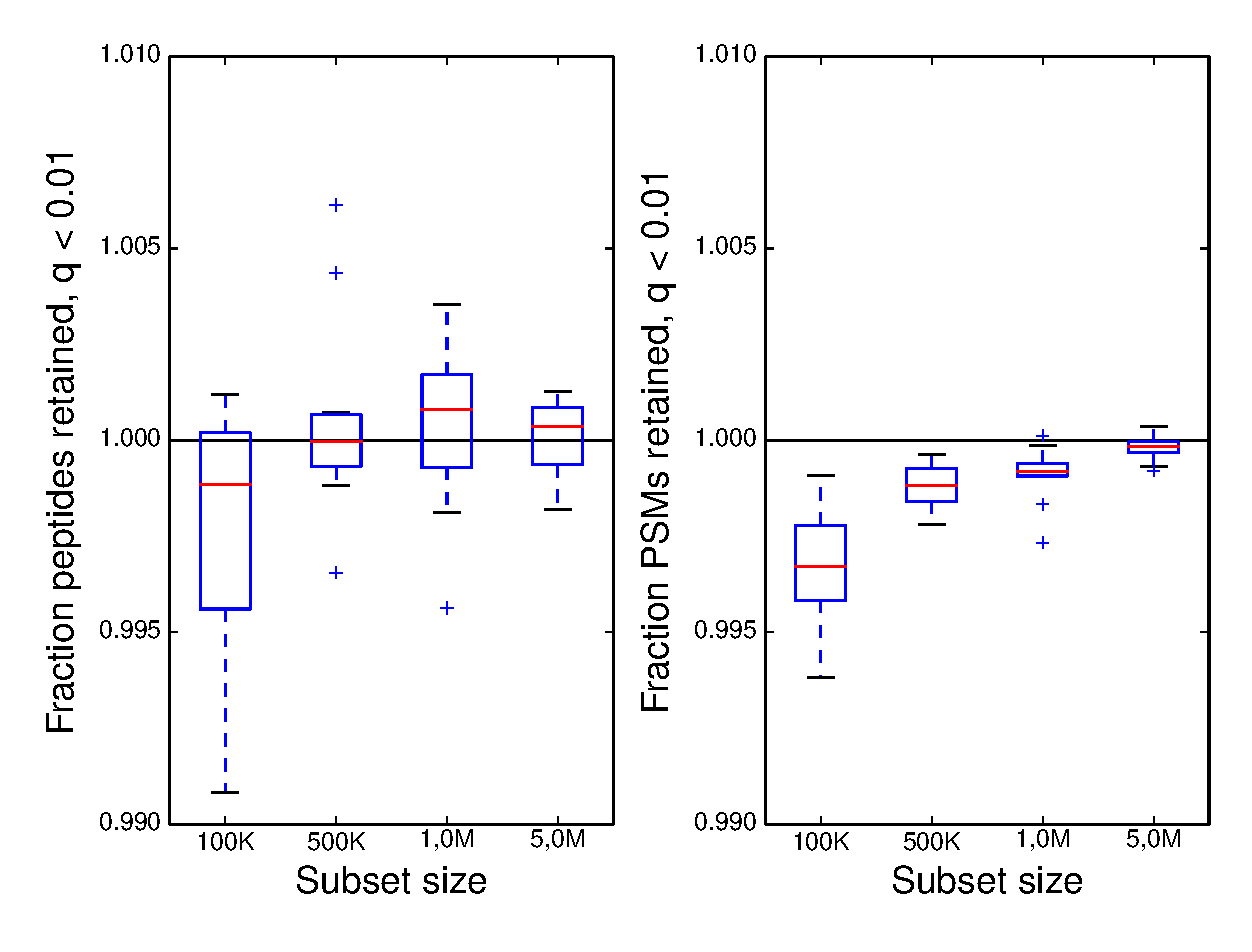
\includegraphics[width=0.6\linewidth]{./img/subset-performance}
\caption{\label{fig:subset}\textbf{SVM training on downsampled data
    retains the performance achieved using the full data set.}  From
  the full Kim data set of $73$ million target+decoy PSMs, we
  evaluated subset sizes of $100\,000, 500\,000, 1\,000\,000$ and
  $5\,000\,000$ PSMs to train the SVMs, repeating this for $10$
  randomized sets, and scored all $73$ million PSMs using the
  resulting support vectors. The figure plots, as a function of data
  set size, the ratio of significant PSMs (left) and peptides (right)
  at a $q$ value threshold of $0.01$ over the same number when using
  the full training set of $73$ million PSMs. The number of 
  significant PSMs and unique peptides does not drop significantly, 
  even for subsets of $100\,000$ PSMs.}
\end{center}
\end{figure}

We used the Kim data set to evaluate the robustness of Percolator's 
SVM classifier to reductions in the size of the training set.  The 
Tide searches of the complete Kim data set against the human 
Swiss-Prot database resulted in $73$ million target and decoy PSMs. 
Post-processing the full data set with Percolator resulted in 
$7\,928\,454$ significant PSMs and $298\,301$ unique target peptides 
at a $q$~value threshold of $0.01$.  To characterize the performance 
of the SVM learning procedure when training on subsets of the PSMs, we 
evaluated performance using training subsets of $100\,000, 500\,000, 
1\,000\,000$ and $5\,000\,000$ PSMs from the Kim data set, using the 
subset training procedure outlined in the Methods section. For each 
training subset size, we calculated the mean and standard deviation 
over $10$ randomized runs of the number of PSMs and peptides with $q$ 
value below $0.01$.

This experiment showed that using subsets as small as $100\,000$ PSMs 
($0.14\%$) for SVM training did not significantly reduce the number of 
inferred peptides and PSMs (Figure \ref{fig:subset}). The standard 
deviation of inferred PSMs across the randomized runs for a fixed 
subset size did seem to increase slightly when taking increasingly 
smaller subsets, but this effect was small. By using a subset of 
$500\,000$ PSMs to train the SVM, Percolator's runtime for producing 
peptide-level results was reduced from almost a full day to less than 
$10$ minutes. Furthermore, the memory consumption dropped from almost 
$100$~GB to just $30$~GB, allowing analysis of this type of 
large-scale data to be done on commodity computers.

\subsection*{Protein-level FDR estimates are poorly calibrated when
  shared peptides are retained}

\begin{figure}
\begin{center}
  \begin{tabular}{cc}
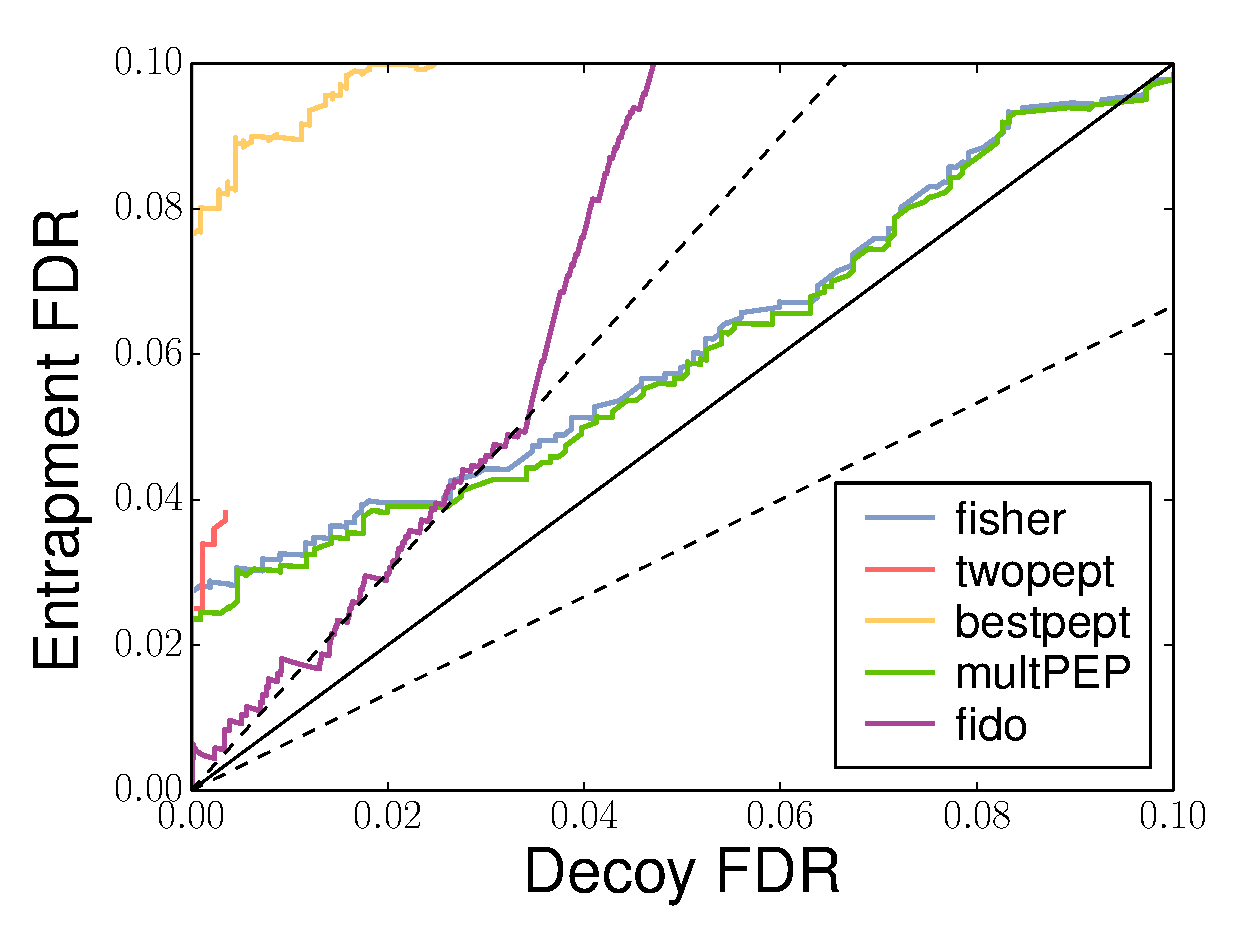
\includegraphics[width=0.45\linewidth]{
./img/shared-pept-accuracy-fdr10-with-fido-exact} &
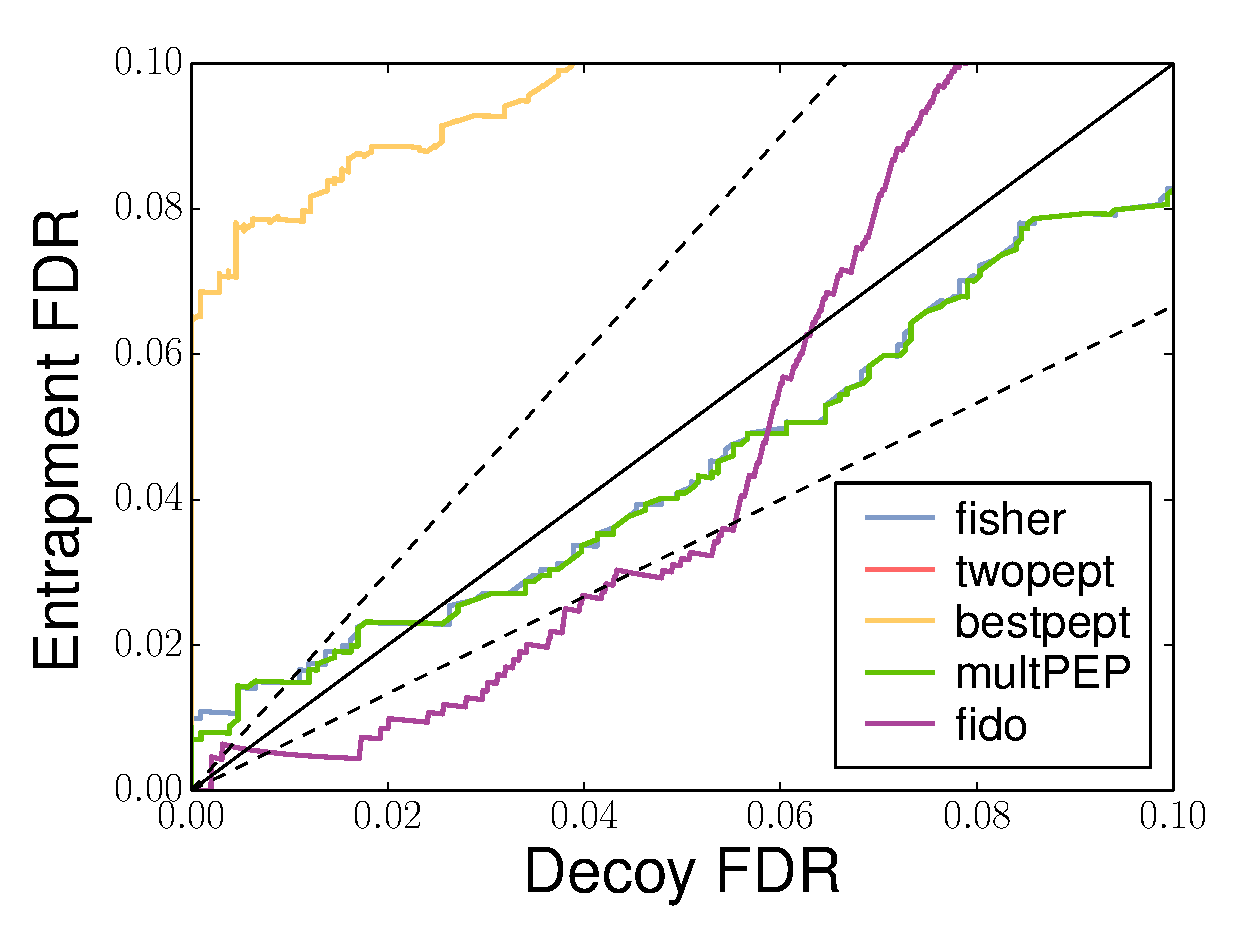
\includegraphics[width=0.45\linewidth]{
./img/shared-pept-accuracy-fdr5-with-fido-exact}\\
  (A) & (B) 
  \end{tabular}
  \begin{tabular}{c}
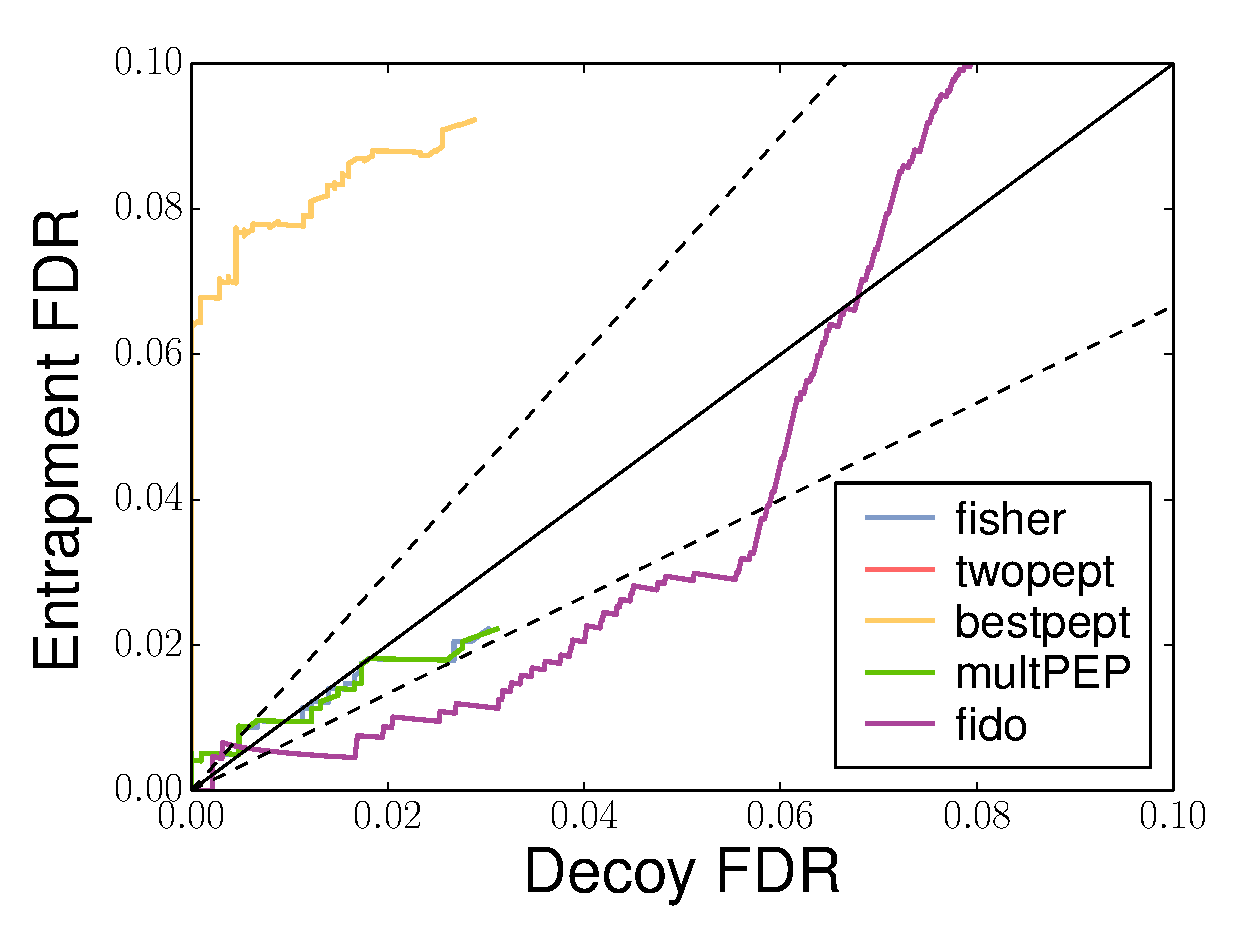
\includegraphics[width=0.45\linewidth]{
./img/shared-pept-accuracy-fdr1-with-fido-exact}\\
  (C)
  \end{tabular}
\caption{\label{fig:shared-accuracy}\textbf{Retaining shared peptides
leads to poor calibration of the decoy model for all the tested
protein inference methods.} The figures plots reported $q$~values from
the decoy model, the decoy FDR, against the fraction of entrapment
proteins in the set of identified target proteins, the observed
entrapment FDR using a peptide-level FDR threshold of $10\%$ (A),
$5\%$ (B) and $1\%$ (C). Dotted lines correspond to $y=1.5x$ and
$y=0.67x$.  For a peptide-level FDR threshold of $10\%$, all five
methods produce anti-conservative FDR estimates, with Fisher's method
and product of PEPs achieving reasonable accuracy above $3\%$ decoy
FDR. For the stricter thresholds of $5\%$ and $1\%$ the FDR estimates
of those two methods are anti-convervative for very low FDRs, but
quickly become conservative for higher FDRs. In comparison, the FDR 
estimates produced by Fido are better calibrated in the very 
low FDR range, but show rather erratic behavior by suddenly switching 
from conservative to anti-conservative estimates around $6\%$ 
entrapment FDR.}
\end{center}
\end{figure}

We assessed the accuracy of decoy-based FDR estimates derived using
four protein inference methods---best-scoring peptide, two-peptide
rule, product of PEPs, and Fisher's method---by analyzing the
hm\_yeast set.  The assessment employed our previously described
sample/entrapment strategy \cite{granholm2013determining}, which
involves comparing the $q$~values reported based on the decoy model,
the ``decoy FDR,'' to the fraction of entrapment proteins in the set
of inferred target proteins, which we call the ``entrapment FDR.''

First, we compared the four protein inference methods while retaining
shared peptides. We grouped proteins that had the same set of
inferred peptides, and also added proteins whose inferred peptides
formed a strict subset of this set to each
group~\cite{nesvizhskii2005interpretation, serang2012review}.  We
performed the experiment three times, varying the peptide-level FDR
threshold (10\%, 5\%, and 1\%) used during the protein grouping
procedure.

This experiment showed that the decoy models based on the reversed 
protein database systematically produce liberal (anti-conservative) 
FDR estimates (Figure \ref{fig:shared-accuracy}). Fisher's method and 
the product of peptide-level PEPs are too liberal for small 
thresholds but manage to provide better estimates above ${\sim}3\%$ 
and ${\sim}1\%$ protein-level FDR for the $10\%$ and $5\%$ 
peptide-level FDR thresholds, respectively. For the two-peptide rule, 
not enough decoy proteins remain to assess if the FDR estimates will 
become more accurate at some point, and the best-scoring peptide 
approach produces dramatically liberal estimates for all thresholds. 
Taking stricter peptide-level thresholds generally improved the 
accuracy for Fisher's method and the product of PEPs. Going down to 
$5\%$ peptide-level FDR still produced anti-conservative protein-level 
FDR estimates in the region below $1\%$ protein-level FDR, but going 
further down to $1\%$ peptide-level FDR actually produced reasonable, 
though still slightly anti-conservative, estimates in that region.

We also investigated the accuracy of the FDR estimates calculated by 
Fido, as implemented in the Percolator package, which would still be a 
viable alternative for smaller data sets. Fido makes use of shared 
peptides and protein grouping, but contrary to the protein grouping 
procedure outlined above only groups proteins with exactly the 
same inferred peptides. It relies on its Bayesian inference engine to 
solve the issue of proteins whose peptides form a strict subset of the 
set of inferred peptides of another protein. Furthermore, Fido 
estimates FDRs by its Bayesian inference engine rather than using a 
decoy FDR, although the decoy FDR curve is in fact used to calibrate 
its parameters. Fido's FDR estimates proved to be better calibrated in 
the region below $1\%$ protein-level FDR than the other four methods, 
but showed divergence from accurate estimates for higher protein-level 
FDRs, both in conservative and anti-conservative direction.

\subsection*{Eliminating shared peptides improves calibration}

\begin{table}
\caption{\label{tab:duplicate-proteins}\textbf{Protein grouping
    increases the number of inferable protein entities.}}
\scriptsize
\begin{center}
\begin{tabular}{lrrr}
\hline
& Swiss-Prot & Swiss-Prot+TrEMBL & Ensembl\\
\hline
Protein sequences & 20\,201 & 69\,714 & 101\,933\\
Peptide sequences & 586\,424 & 664\,801 & 672\,519\\
Proteins with protein-specific peptides & 19\,938 & 52\,834 &
49\,871\\
Protein groups & 20\,104 & 58\,605 & 68\,370\\
Protein groups with protein group-specific peptides & 19\,978 &
54\,292 & 58\,929\\
\hline
\end{tabular}
\end{center}
\end{table}

We hypothesized that these calibration problems arise from the
peptides that are shared between different proteins in the database.
Accordingly, we next considered an approach that discards shared
peptides, retaining only those that are unique to a single protein.
To reduce the effect of fictitious shared peptides that correspond to
protein fragments or other truncated protein forms, we used the
approach to handling shared peptides from Nesvizhskii {\em et
  al.}~\cite{nesvizhskii2003statistical}. Here, proteins are mapped to
their theoretical proteolytically digested peptides, rather than their
experimentally discovered peptides, and two proteins $A$ and $B$ are
merged into a group if protein $A$'s peptides are a superset of
protein $B$'s peptides or vice versa.  We then retain the peptides
that are unique to a protein group, rather than to a single protein.
A side effect of this change is that, in contrast to the procedure
used in Figure~\ref{fig:shared-accuracy}, we do not have to apply any
peptide-level FDR threshold because all protein grouping is done
before the data is observed.

We applied this approach to several protein databases and showed 
empirically that including the protein grouping step increases the 
number of protein entities, {\em i.e.}, single proteins or protein 
groups, with a peptide uniquely identifying it. The experiment 
involved performing a fully tryptic digestion, with no missed 
cleavages, of three human protein databases---Swiss-Prot, 
Swiss-Prot+TrEMBL, and Ensembl---considering peptides with lengths of 
6--50 amino acids. TrEMBL and Ensembl contain many proteoforms and 
therefore benefit significantly from this particular protein grouping 
approach in terms of number of identifiable protein entities (Table 
\ref{tab:duplicate-proteins}). Note that, unfortunately, some protein 
groups will remain unidentifiable, because all their peptides are 
shared by at least two different protein groups. The in-silico protein 
digestion and subsequent grouping required only $15$ seconds for the 
Swiss-Prot database and $4$ minutes for the Swiss-Prot + TrEMBL 
database.

\begin{figure}
\begin{center}
\begin{tabular}{cc} 
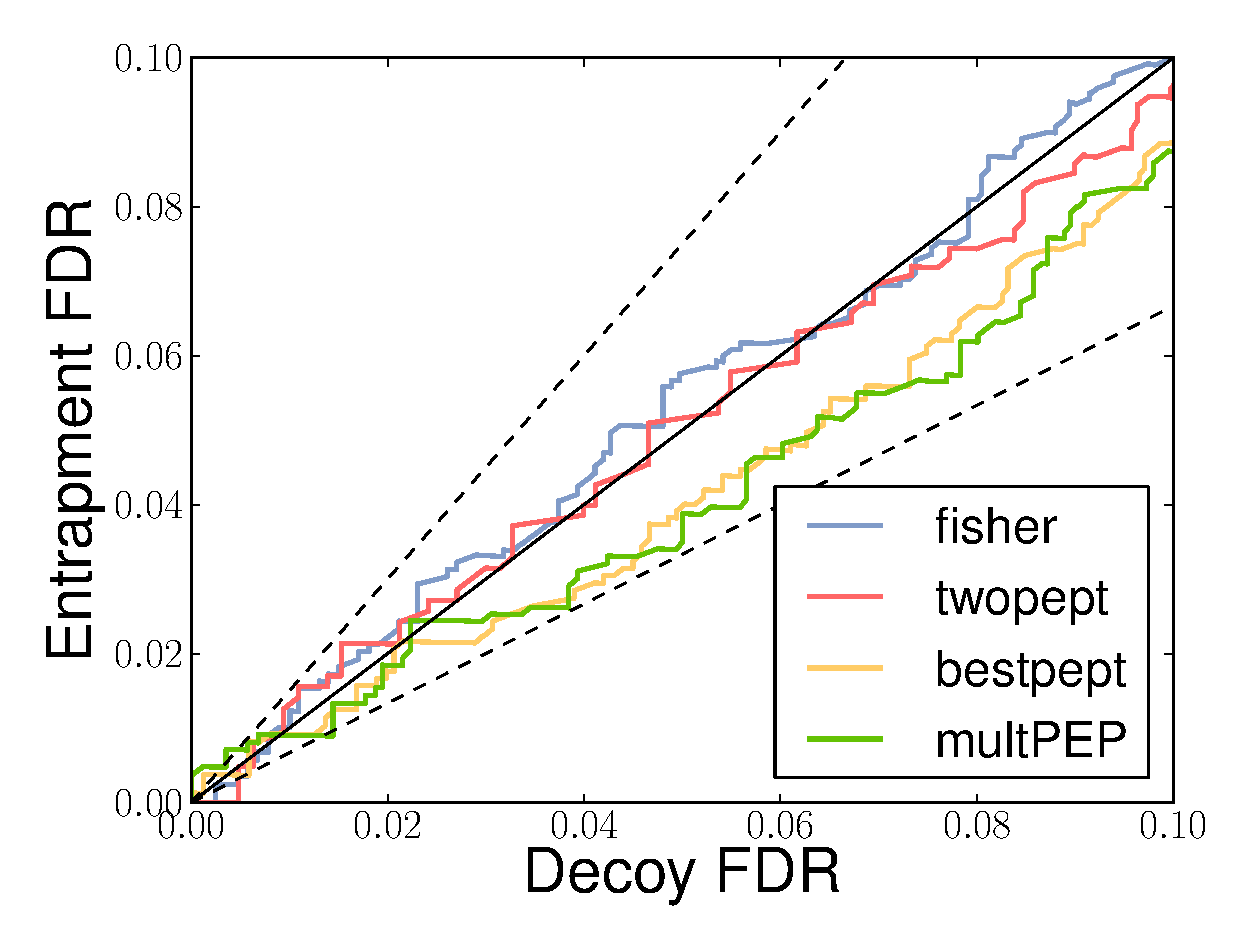
\includegraphics[width=0.45\linewidth]{./img/unique-pept-accuracy} &
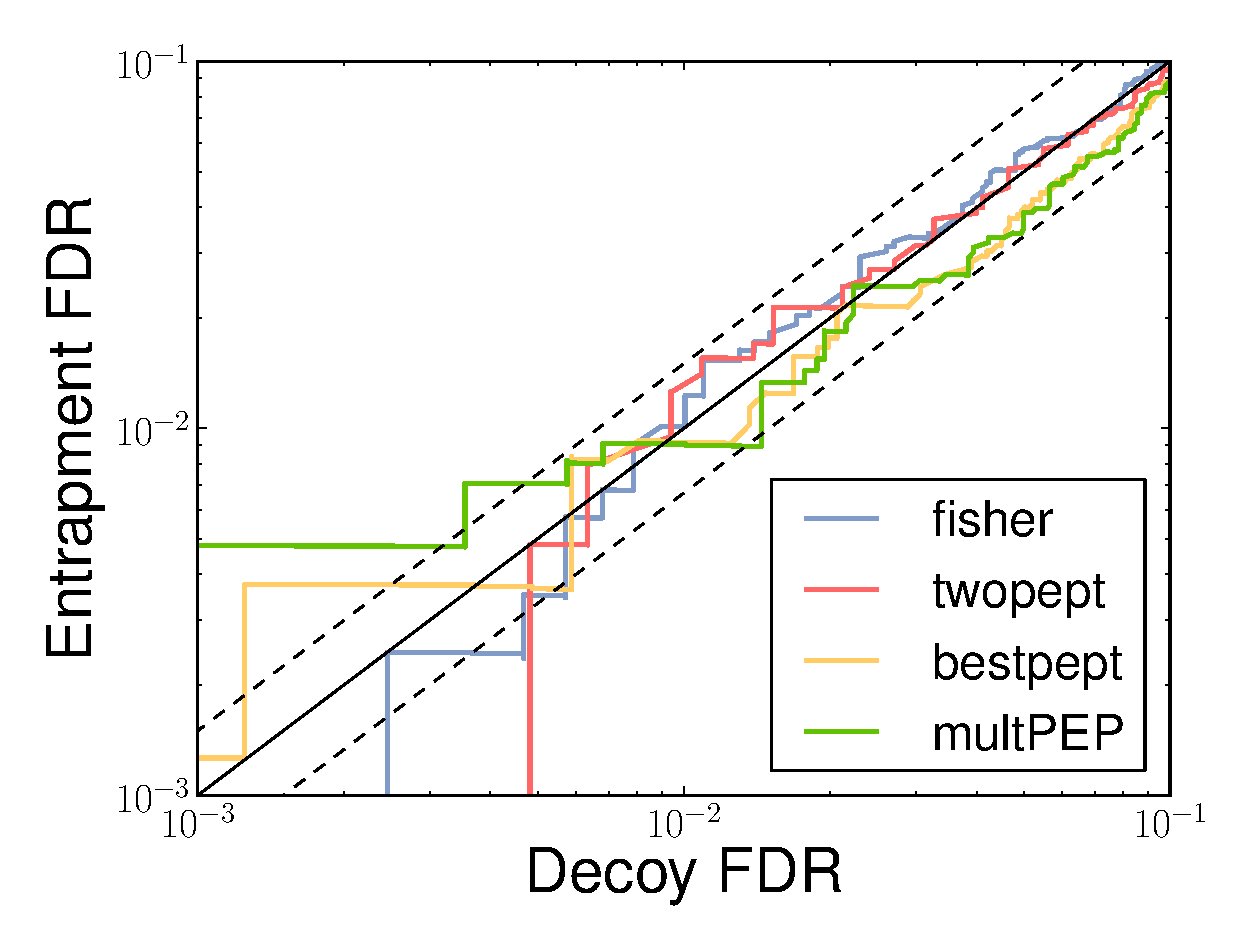
\includegraphics[width=0.45\linewidth]{./img/unique-pept-accuracy-log}
\\
(A) & (B)
\end{tabular}
\caption{\label{fig:unique-accuracy}\textbf{Using only protein-unique
    peptides gives accurate estimates of the protein-level FDR.}  (A)
  The figure plots the decoy FDR against observed entrapment FDR.  All
  four methods produce accurate FDR estimates. (B) A logarithmic plot
  of the region $[0.001, 0.1]$ with the same axes as in (A).}
\end{center}
\end{figure}

Having eliminated the shared peptides, we returned to our
sample/entrapment strategy for estimating the accuracy of
protein-level FDR estimates.  In this new setting, all four methods
now gave accurate protein-level FDR estimates (Figure
\ref{fig:unique-accuracy}A).  Zooming in on the low FDR region (Figure
\ref{fig:unique-accuracy}B) showed that the protein-level FDR
estimates break down somewhere in the $[0.001, 0.01]$ range,
presumably due to the low density of decoy proteins in that region.
From these results, it became clear that taking only unique peptides,
together with the protein grouping approach from Nesvizhskii {\em et
  al.}, would be the most robust choice, regardless of the protein
inference method.


\subsection*{Selection of a protein inference strategy}

% \begin{figure}
% \begin{center}
% \begin{tabular}{ccc} 
% \includegraphics[width=0.3\linewidth]
%   {./img/shared-pept-performance-fdr10} &
% \includegraphics[width=0.3\linewidth]
%   {./img/shared-pept-performance-fdr5} &
% \includegraphics[width=0.3\linewidth]
%   {./img/shared-pept-performance-fdr1}\\
% (A) & (B) & (C)
% \end{tabular}
% \caption{\label{fig:shared-performance}\textbf{Comparison ofprotein
% inference methods when retaining shared peptides.} We plotted the
% number of sample proteins, which can be considered an estimate for the
% number of true inferences, against the observed entrapment FDR using a
% peptide-level FDR threshold of $10\%$ (A), $5\%$ (B) and $1\%$ (C).
% Whereas Fisher's method, the product of peptide-level PEPs and the two
% peptide rule initially pick up many sample proteins, the best-scoring
% peptide approach immediately breaks down. Stricter peptide-level
% thresholds increase the number of protein detections at $1\%$
% protein-level FDR for the $3$ other methods.}
% \end{center}
% \end{figure}

\begin{figure}
\centering
\begin{tabular}{ccc}
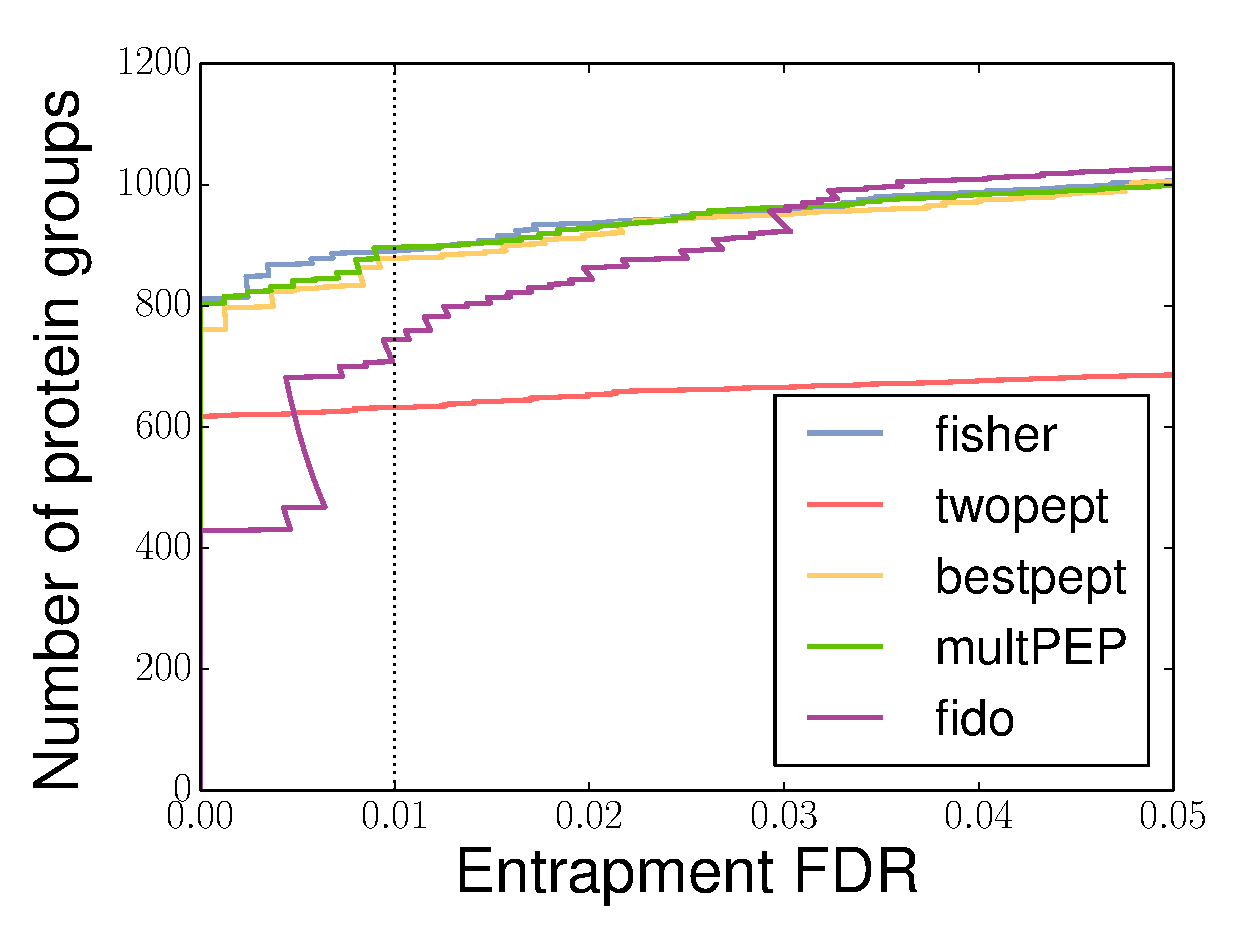
\includegraphics[width=0.45\linewidth]{
./img/unique-pept-performance-with-fido-exact} &
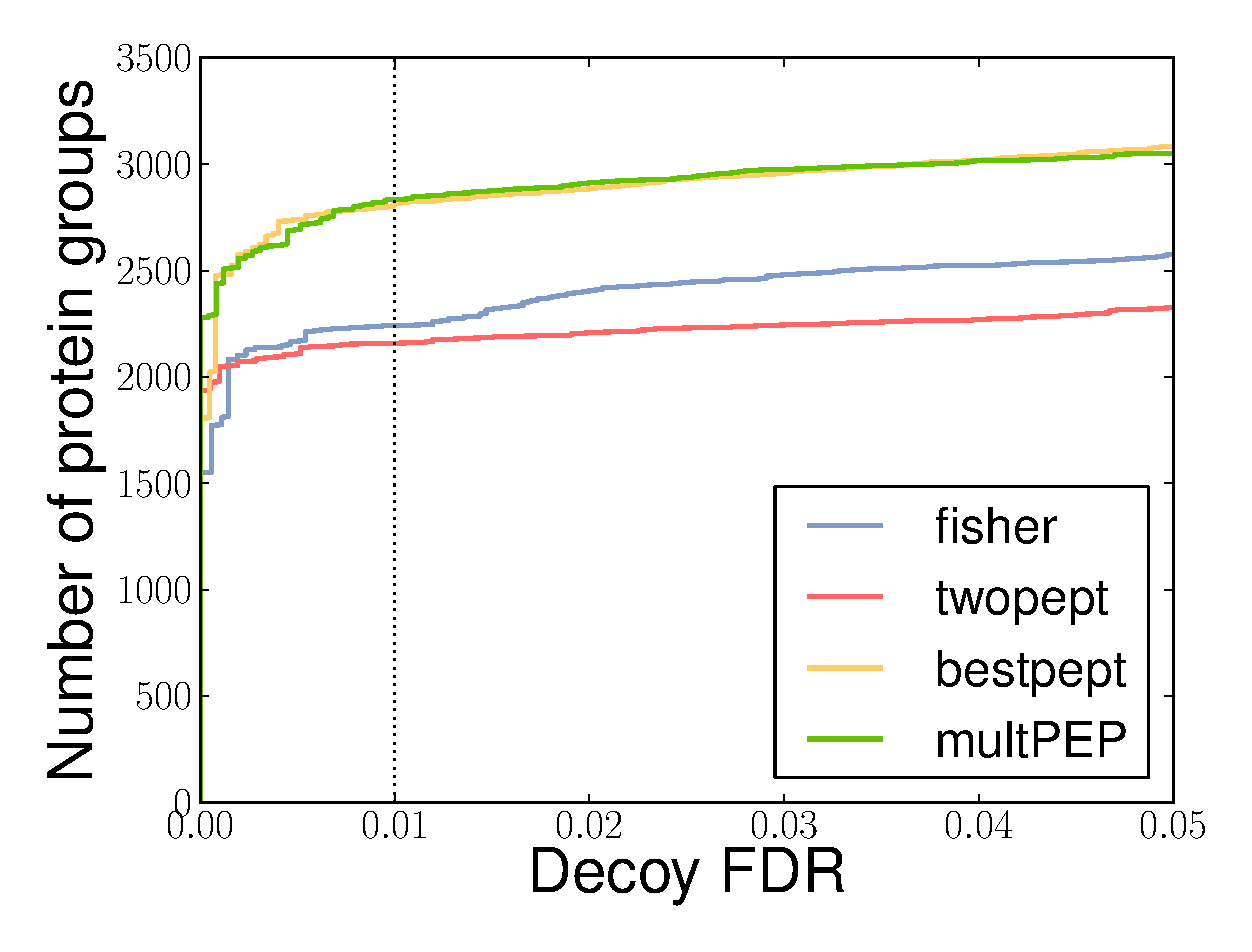
\includegraphics[width=0.45\linewidth]
{./img/wu-ipi-performance}\\
(A) & (B)\\
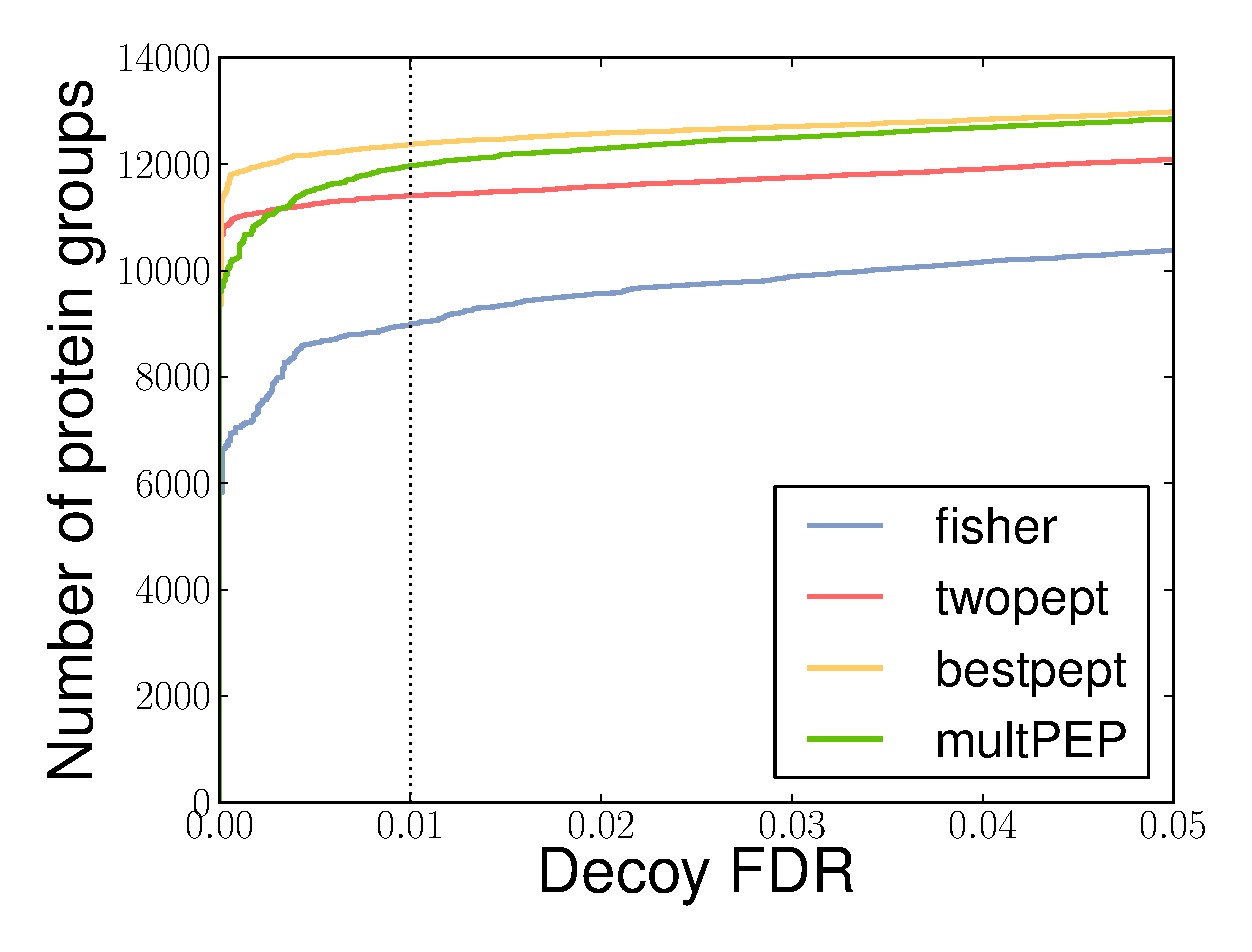
\includegraphics[width=0.45\linewidth]
{./img/kim-swissprot-performance} &
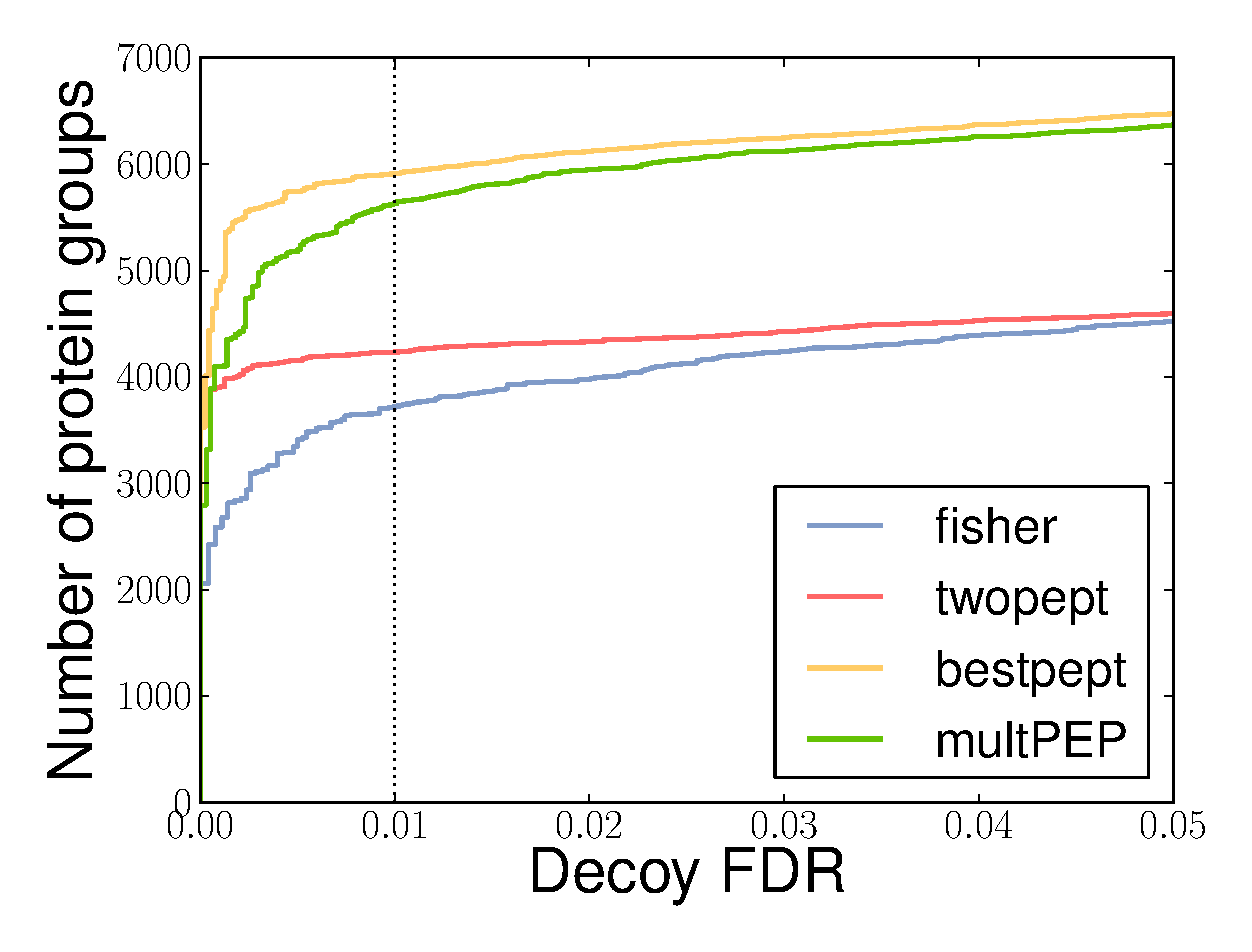
\includegraphics[width=0.45\linewidth]
{./img/kim-uniprot-performance}\\
(C) & (D)
\end{tabular}
  \caption{{\bf Comparison of protein inference methods.} (A) The
figure plots the number of accepted protein groups against the 
observed entrapment FDR for the hm\_yeast set. Fisher's method, the 
product of peptide-level PEPs and the best-scoring peptide approach 
all perform about equally, while Fido and the two-peptide rule are 
much less sensitive. We used a peptide-level threshold of $5\%$ 
for Fido in this plot, but thresholds of $10\%$ and $1\%$ gave very 
similar results. (B) A plot of the number of accepted protein groups 
against the decoy FDR for the Wu data set. The product of 
peptide-level PEPs and the best-scoring peptide approach perform best, 
while the two-peptide rule and Fisher's method inferred far fewer 
protein groups. (C,D) Same axes as in (B) but for the Kim data set, 
searched using the Swiss-Prot (C) and Swiss-Prot+TrEMBL (D) databases. 
The best-scoring peptide approach inferred the most protein groups 
for both databases.}
  \label{fig:power}
\end{figure}

Finally, we compared the number of inferred proteins as a function of 
the observed entrapment FDR for the different inference methods.  For 
the hm\_yeast data set, Fido and the two-peptide rule were clearly 
performing worse than the others (Figure~\ref{fig:power}A). We then 
repeated the assessment on the much larger Wu and Kim data sets, using 
the IPI database for the Wu set and two different databases 
(Swiss-Prot and Swiss-Prot+TrEMBL) for the Kim set. Even for such 
large-scale data, all four protein inference methods took less than a 
minute of processing time due to their simplicity. We looked at the
number of inferred protein groups at $1\%$ reported protein-level FDR
(Figure~\ref{fig:power}B-D). For the Wu data set, the multiplication
of PEPs and the best-scoring peptide approach performed best. Fisher's
method inferred far fewer protein groups than the other three methods,
possibly due to incorrect peptides dragging down the $p$ value of
correct protein groups. For the Kim data set, the best-scoring peptide
approach inferred the most protein groups for both databases with a
$3\mbox{--}5\%$ margin over the second-best method. Although the many
proteoforms in the TrEMBL database caused a large drop in the number
of protein groups for all methods, the relative ranking of methods was
consistent in both sets of results. 

\begin{figure}
\centering
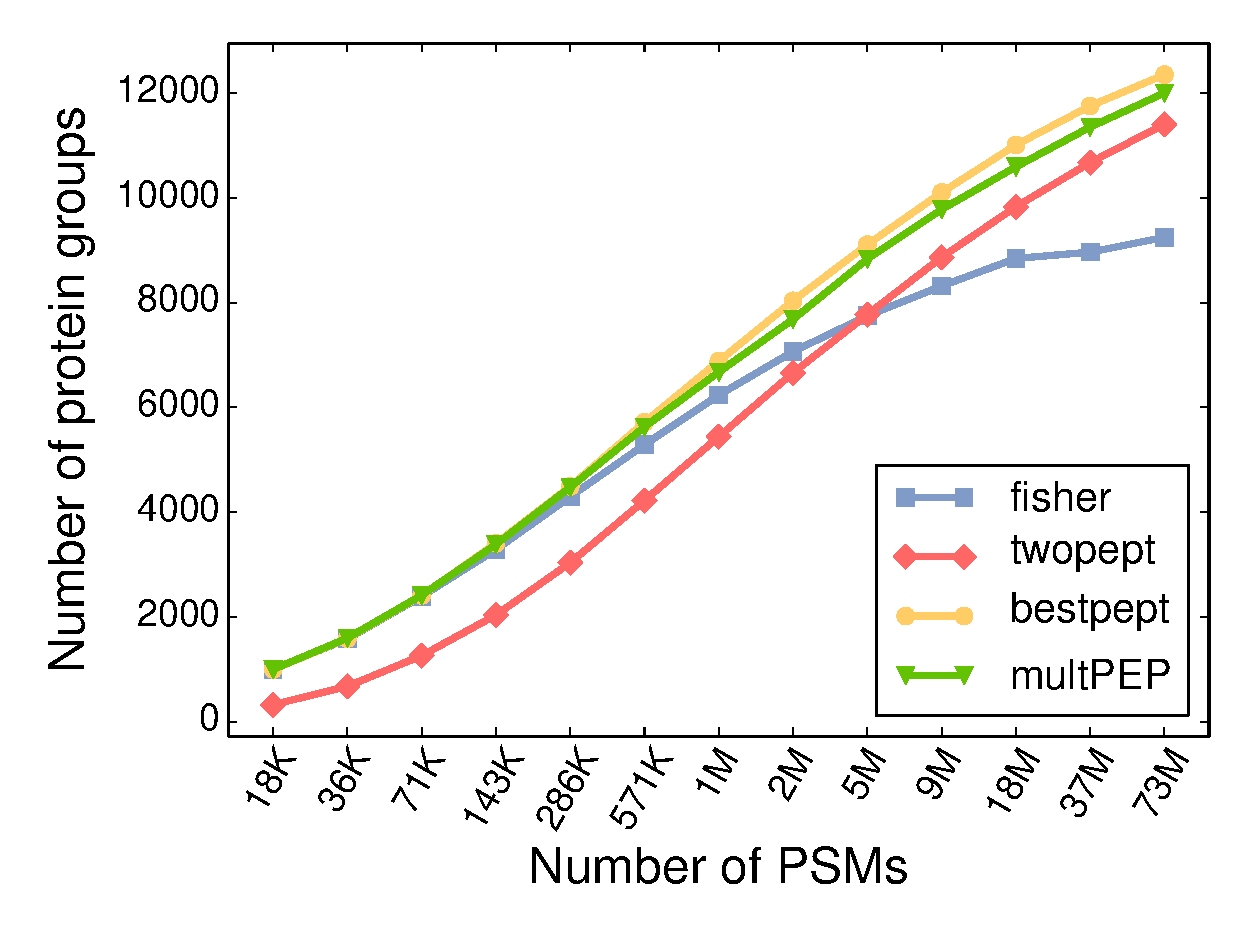
\includegraphics[width=0.6\linewidth]
{./img/kim-downsampling-performance}
  \caption{{\bf Sample size dependence of protein inference methods.}
    We plotted the average number of accepted protein groups at $1\%$
    protein-level FDR over triplicate random subsets of using
    different subset sizes of the Kim set matched to the Swiss-Prot
    database.  The number of PSMs was reduced from the original $73$
    million PSMs with factors of $2$ until $18$K PSMs. Fisher's
    method, the product of peptide-level PEPs and the best-scoring
    peptide approach all perform about equally until $200$K
    PSMs. Above this number of PSMs, the best-scoring peptide approach
    outperforms all the other methods.}
  \label{fig:power-downsample}
\end{figure}

Finally, we looked at the number of inferred protein groups for random 
subsets of the Kim data set (Figure~\ref{fig:power-downsample}).  For 
small data sets, all methods except the two-peptide rule perform about 
equally. However, as the data sets get larger, the best-scoring 
peptide approach starts to show its advantage. Overall, we concluded, 
in agreement with Savitski {\em et al.} \cite{savitski2015scalable}, 
that the best-scoring peptide approach yielded the best overall 
performance. We therefore implemented this protein inference method in 
the latest Percolator package.

% \begin{table}
%   \begin{center}
%     \begin{tabular}{lrr}
%     \hline
%     partial digestion & Swiss-Prot & Swiss-Prot+TrEMBL\\
%     \hline
%     Best-scoring peptide & 12\,370 & 5\,909\\
%     Product peptide-level PEPs & 11\,968 & 5\,626\\
%     Two-peptide rule & 11\,409 & 4\,231\\
%     Fisher's method & 8\,964 & 3\,717\\
%     \hline
%     \end{tabular}
%   \end{center}
% \caption{\label{tab:pandey-stats}\textbf{Using the best-scoring
%   peptide as a protein's representative inferred the most protein
%     groups.} We examined the number of protein inferences for the
%   four protein inference method using only peptides unique to one of
%   the protein groups formed by the approach from Nesvizhskii {\em et
%     al.}. }
% \end{table}

\section*{Discussion}

We demonstrated that Percolator 3.0 can calculate accurate
protein-level FDRs on a human proteome-scale study, in this case $73$
million PSMs, in a matter of minutes on a commodity computer.

The downsampling approach for SVM training on a subset of the PSMs 
shows great stability even when only sampling a tiny fraction, as 
small as $100,000$ PSMs, {\em i.e.} $0.14\%$ of the original set of 
$73$ million PSMs.  The Kim data set might not be as representative 
for other types of studies that have greater heterogeneity, but it 
seems likely that the downsamping strategy will work well as long as 
the selected subset of PSMs contains a sufficient number of positive 
training examples.

The most successful protein inference method turned out to be the one
where proteins were grouped by their theoretical peptide sets and only
the best-scoring peptide was considered. In this approach, the score
assigned to a protein essentially ignores the majority of the PSMs,
something that may feel quite unsatisfying. On the other hand,
including evidence from other, lower-scoring peptide inferences is
difficult because it often involves lumping incorrect peptide
inferences into correct protein inferences.  This problem can clearly
be seen in the poor performance of Fisher's method for combining $p$
values on the Wu and Kim data sets. Setting peptide-level thresholds
can actually bring Fisher's method up to par with the best-scoring
peptide approach (data not shown). However, this modification does not
produce significantly more protein inferences, while introducing an
extra parameter that needs to be set correctly.

With regards to the discarded shared peptides, large-scale studies
give us the luxury of deep coverage, therefore inferring many
peptides that are unique to a protein. This mitigates the problem of
ignoring shared peptides and makes the task of protein inference much
simpler and intuitive.

The protein grouping method employed here still suffers from the 
problem that an inference of a protein group leaves open the question 
which proteins in the group are actually correct. Here, we interpreted 
it using the null hypothesis that all proteins in the group are 
incorrect, {\em i.e.}, an inferred protein group means that we expect 
at least one of the proteins to be correct, but we are agnostic about 
which one. Compared to the conventional protein grouping approach, 
which is based on inferred peptides instead of the full set of 
theoretical peptides, the groups produced by our method are much 
smaller. For the Swiss-Prot database, virtually all protein groups 
contained only $1$ protein and for the Swiss-Prot + TrEMBL database 
they typically contained just $1$ or $2$ proteins. Consequently, 
ambiguity about which specific proteins are present is much rarer.  
Furthermore, if genes, rather than proteoforms, are the entities of 
interest, then using databases with few proteoforms such as Swiss-Prot 
should do the job.

We have not extensively tested our new protein inference functionality 
on smaller data sets. However, based on the results for the hm\_yeast 
set and the small random subsets of the Kim set, we believe that the 
estimated FDRs will remain accurate and that it is unlikely that any 
of the other evaluated protein inference methods will identify many 
more proteins.

The construction of the entrapment database in this study should be
considered as a rather crude approximation of true experimental
settings and could be improved upon in future work. While our approach
does conserve homologs by shuffling peptide rather than protein
sequences, the method only allows for simulation of fully-tryptic
peptides without missed cleavages.  Furthermore, the mechanism that
creates shared peptides between sample and entrapment database does
not attempt to model homology.  In our approach, the shared peptides
are randomly distributed over all proteins, whereas in practice we can
expect some portion of proteins to share multiple peptides and many
proteins to have no shared peptides at all. The rate of shared
peptides---$4\%$, modeled after the Swiss-Prot yeast database---is
also a good approximation of the shared peptide rate of the Swiss-Prot
human database. However, the shared peptide rate in the
Swiss-Prot+TrEMBL database is much higher, with over $60\%$ of the
peptides being shared by at least two proteins.  Modeling this level
of redundancy could result in significantly different outcomes.

For our largest evaluated data set, the $73$ million PSMs of the Kim 
data set, the combined runtime for Percolator 3.0, {\em i.e.} from 
PSMs to protein-level FDRs, was $10$ and $15$ minutes for the 
Swiss-Prot and Swiss-Prot + TrEMBL database respectively. We realize 
that other parts of the shotgun proteomics analysis pipeline might 
still have significantly higher computing requirements than 
Percolator, but fortunately these can often readily be parallelized as 
the runs can be analyzed independently. However, as we have pointed 
out elsewhere, obtaining significance measures per run or data set and 
combining them afterwards is not at all straightforward and should be 
handled with great caution~\cite{serang2015solution}. This new version 
of Percolator allows the user to easily obtain statistical 
significance measures on aggregated data from a great number of runs 
without running this risk.

\section*{Acknowledgements}

Part of the computations were performed on resources provided by the
Swedish National Infrastructure for Computing (SNIC) at Uppsala
Multidisciplinary Center for Advanced Computational Science (UPPMAX).
This work was supported by National Institutes of Health award
P41~GM103533.

\bibliographystyle{plain}
\bibliography{percolator}

\end{document}
